\documentclass{beamer}
\usepackage[utf8]{inputenc}
\usepackage[T1]{fontenc}
\usepackage{graphicx}
\usepackage{tcolorbox}
\usepackage{hyperref}
\hypersetup{
    colorlinks=true,
    linkcolor=pink,
    urlcolor=cyan,
    urlbordercolor=cyan,
}
\graphicspath{ {./images/} }

\usetheme{Arguelles}

\title{Tutorial 3}
\subtitle{CS3241 Computer Graphics (AY22/23)}
\date{\today}
\author{Wong Pei Xian}
\institute[]{\email{e0389023@u.nus.edu}}

\begin{document}

\frame[plain]{\titlepage}

\section{Question 1}

\begin{frame}
    \frametitle{Question 1a}
    Given three points A, B, and C in 3D space, write an expression for the \textbf{normal vector}
    of the plane that contains the three points.
\end{frame}

\begin{frame}
    \frametitle{Normal vector}

    \begin{center}
        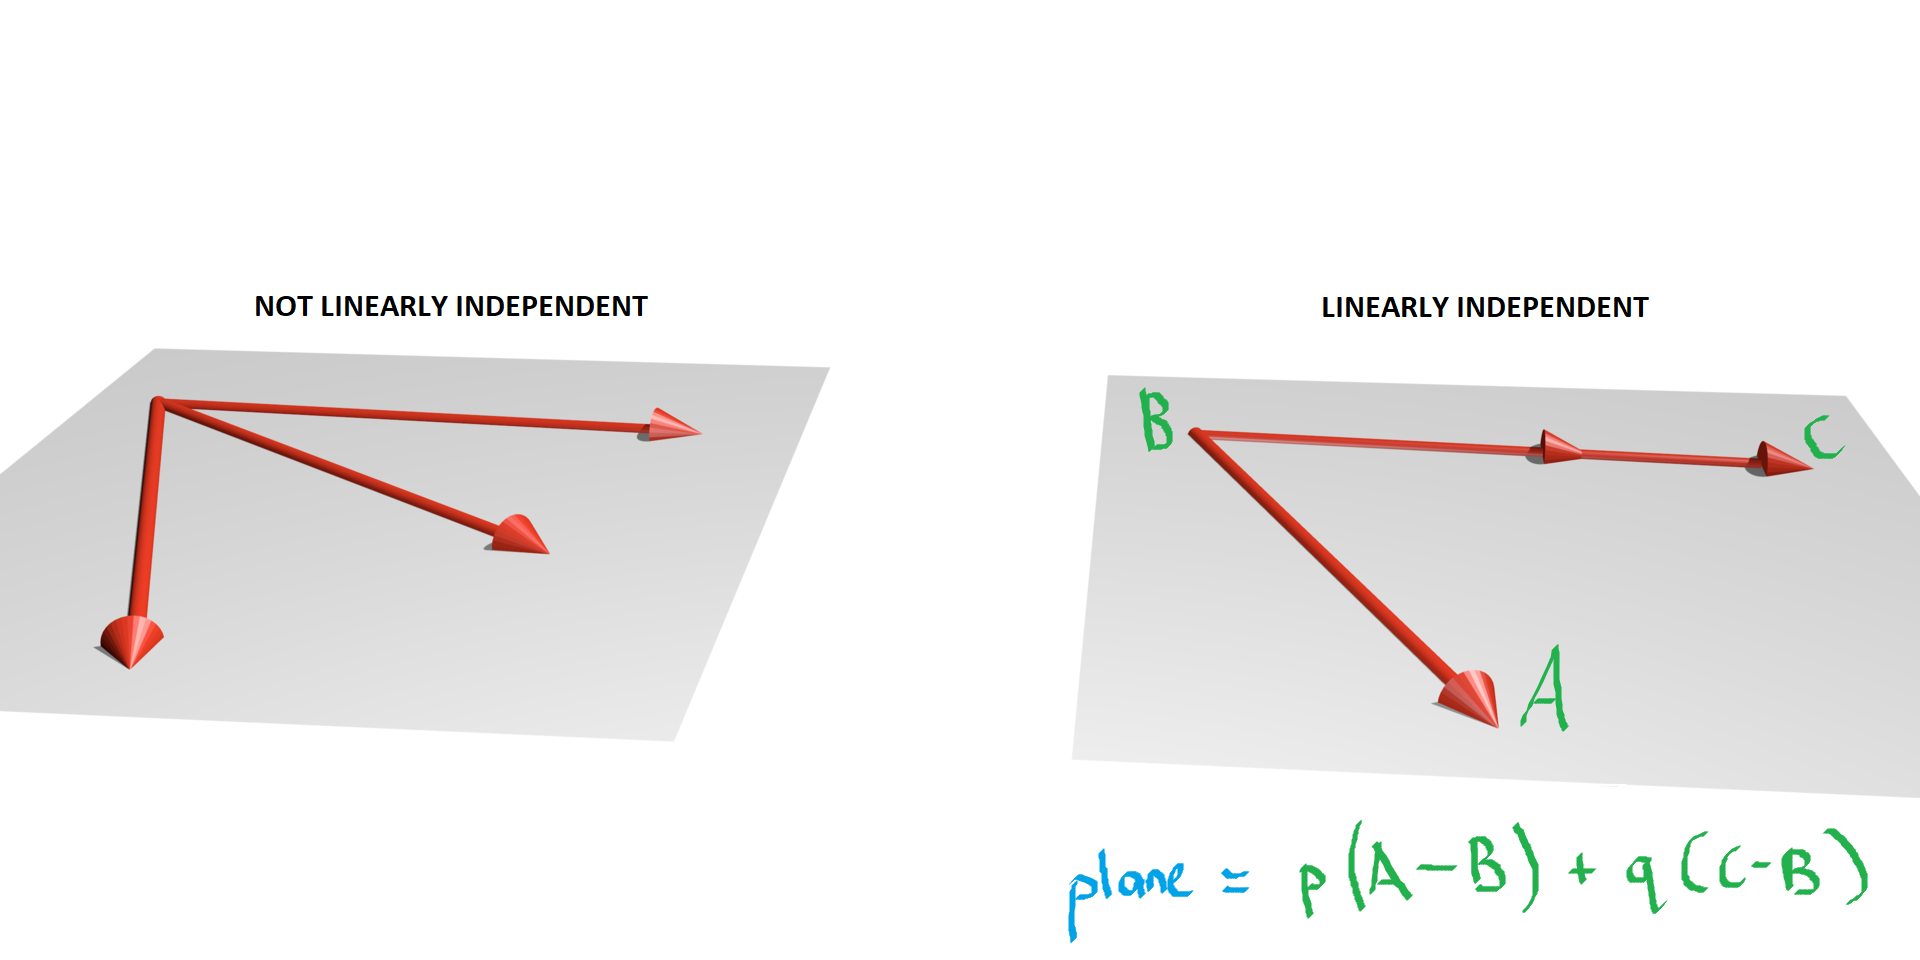
\includegraphics[scale=0.25]{1920px-Vec-dep.png}
    \end{center}

    The \textbf{linear combination} of any two \textbf{linearly independent} vectors forms a plane.

\end{frame}

\begin{frame}
    \frametitle{Question 1b}

    Given a point $R = [r_x \  r_y \  r_z]^T$ on a plane $\Pi$ and a normal vector 
    $n = [n_x \  n_y \  n_z]^T$ of the plane, write the implicit-form equation of 
    the plane in the form $ax + by + cz + d = 0$.

\end{frame}

\begin{frame}
    \frametitle{Implicit form}

    \begin{center}
        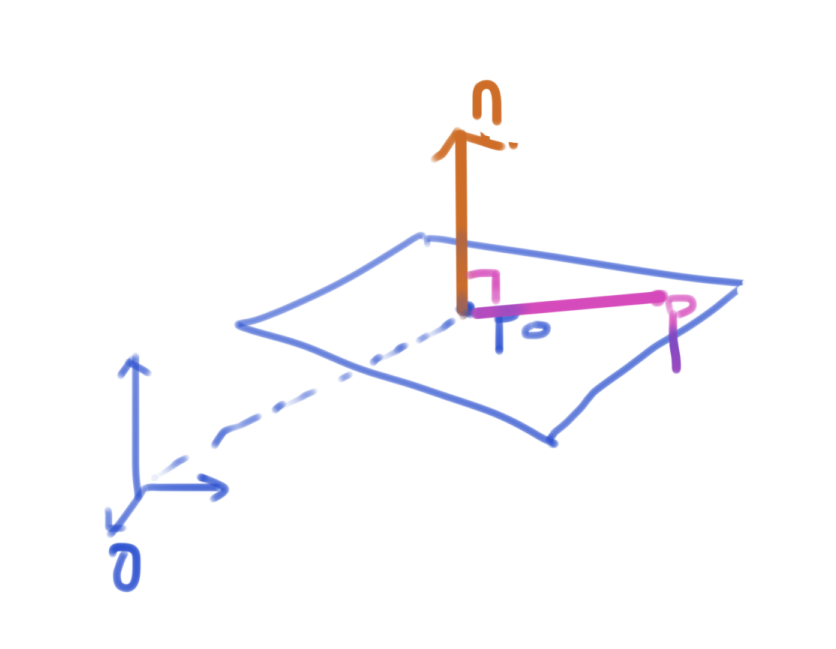
\includegraphics[scale=0.4]{plane-def.png}

        \begin{eqnarray}
            n \cdot ([x \  y \  z]^T - R) &= 0 \\ 
            n_x x + n_y y + n_z z - n\cdot R &= 0
        \end{eqnarray}
    \end{center}

\end{frame}

\begin{frame}
    \frametitle{Question 1c}
    
    What is the perpendicular distance of the point $Q$ from the plane $ax + by + cz + d = 0$?

\end{frame}

\begin{frame}
    \frametitle{Perpendicular distance of point to plane}

    Let $Q = [q_x \  q_y \  q_z]^T$. Then the distance $D$ from point to plane is 

    \begin{eqnarray}
        D = \left| \frac{aq_x + aq_y + aq_z + d}{\sqrt{a^2 + b^2 + c^2}}\right|
    \end{eqnarray}

\end{frame}

\section{Question 2}

\begin{frame}
    \frametitle{Question 2a}

    What does the homogenous coordinates $[6, 4, 2, 0.5]^T$ represent?

\end{frame}

\begin{frame}
    \frametitle{Question 2a}

    What does the homogenous coordinates $[6, 4, 2, 0.5]^T$ represent?

    \begin{tcolorbox}
        \begin{eqnarray*}
            & \left[
            \begin{matrix}
                x & y & z & w
            \end{matrix} 
            \right]\\
            = & \left[
            \begin{matrix}
                x/w & y/w & z/w & 1
            \end{matrix}
            \right]
        \end{eqnarray*}
    \end{tcolorbox}
    

\end{frame}

\begin{frame}
    \frametitle{Question 2b}

    Why does OpenGL (and many other graphics APIs) use homogeneous coordinates to represent points?

\end{frame}

\begin{frame}
    \frametitle{Why homogenous coordinates?}

    \begin{enumerate}
        \item Different representations for points aand vectors.
        \item $4 \times 4$ Matrix multiplication
        \item Perspective projection with matrix mult. and \textit{perspective division}.
    \end{enumerate}
    
\end{frame}

\begin{frame}
    \frametitle{Point vector distinguishing}

    For \textbf{vector}; $w = 0$ \quad e.g. $\left[ \begin{matrix}
        x & y & z & 0
    \end{matrix} \right]$.

    For \textbf{point}; $w = 1$ \quad e.g. $\left[ \begin{matrix}
        x & y & z & 1
    \end{matrix} \right]$.

    \begin{tcolorbox}
        In this week's lecture, you will learn that to transform \textbf{normal vectors} instead of points,
        we use the matrix
        \begin{eqnarray*}
            M_n = (M_t^{-1})^T
        \end{eqnarray*}
        where $M_t$ is the upper left $3 \times 3$ submatrix.
    \end{tcolorbox}

\end{frame}

\section{Question 3}

\begin{frame}
    \frametitle{Question 3}

    Which of the followings is the matrix that rotates objects about the fixed 3D point 
    $[2 \  3 \  4]^T$, where the rotation axis is parallel to and in the same direction 
    as the x-axis, and the rotation angle is $\theta$? 

    \begin{center}
        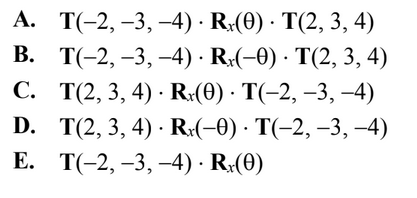
\includegraphics[scale=0.6]{q3-options.png}
    \end{center}

\end{frame}

\begin{frame}
    \frametitle{Things to note about transformation}


    \begin{center}
        
\includegraphics[scale=0.4]{order-of-trans.png}
    \end{center}

\end{frame}

\begin{frame}
    \frametitle{Things to note about transformation}


    \begin{center}
        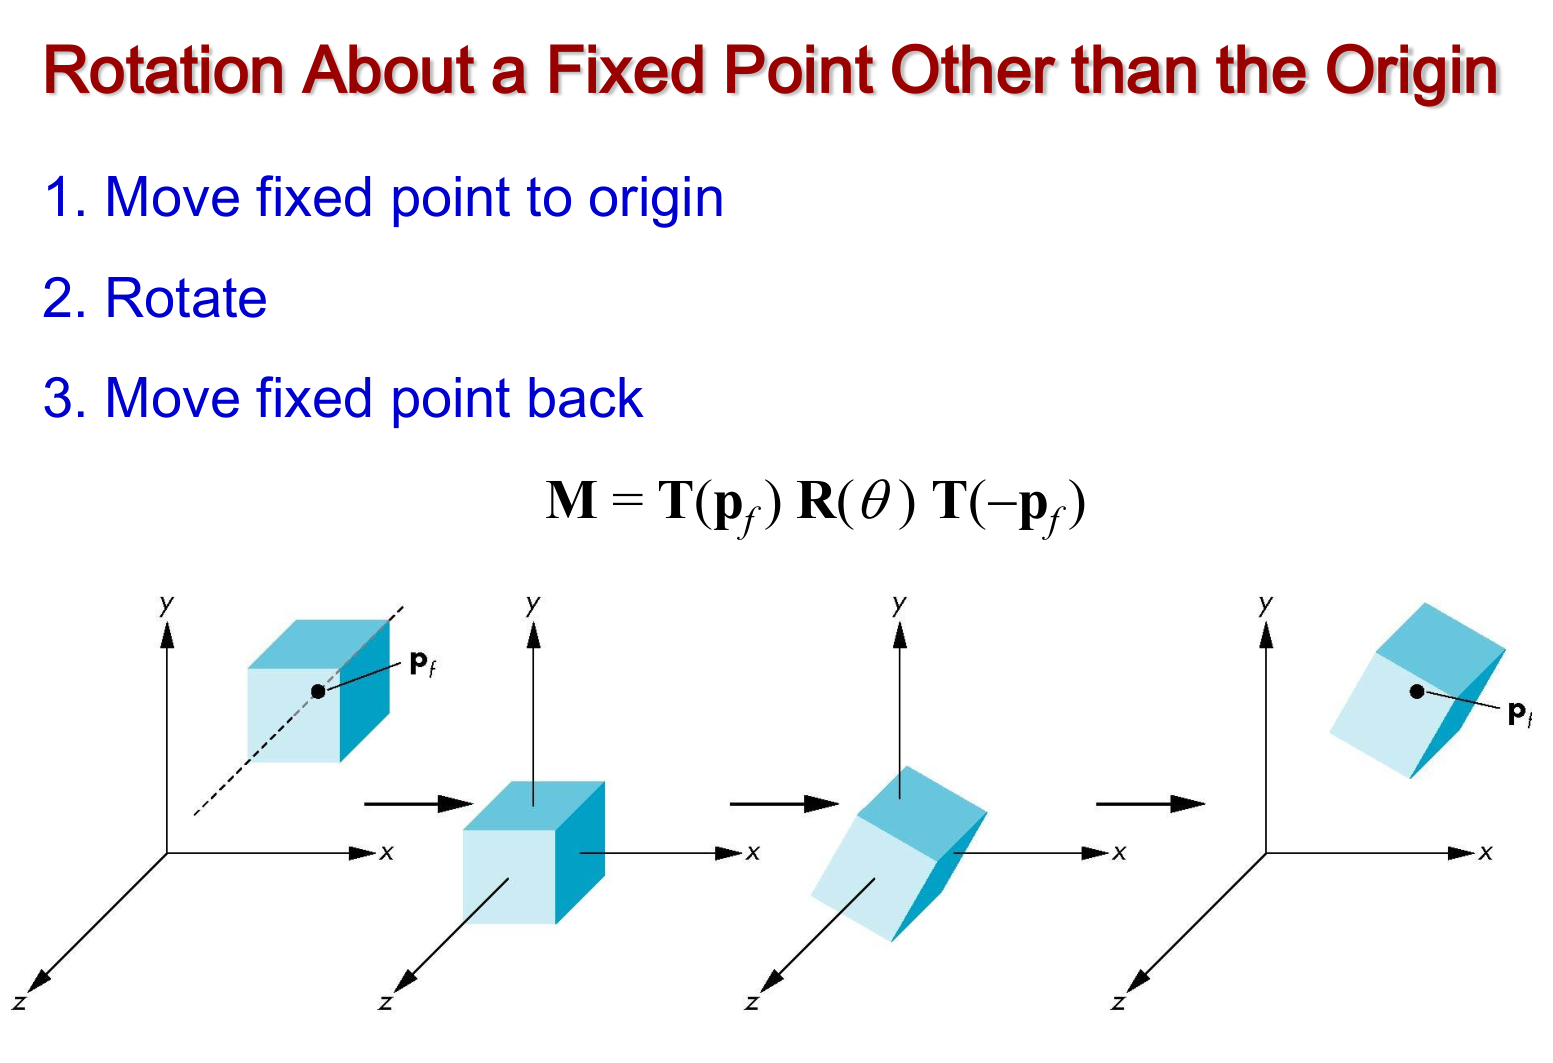
\includegraphics[scale=0.3]{rotate-about-fixed-pt.png}
    \end{center}

    \begin{tcolorbox}
        Ans: $T(2,3,4) \cdot R(\theta) \cdot T(-2, -3, -4)$.
    \end{tcolorbox}

\end{frame}

\section{Question 4}

\begin{frame}
    \frametitle{Question 4}

    What is the inverse matrix of 

    \begin{center}
        $$ M = 
        \left[
        \begin{matrix}
            s_1 r_{11} & s_1 r_{12} & s_1 r_{13} & t_1\\
            s_2 r_{22} & s_2 r_{22} & s_2 r_{23} & t_2\\
            s_3 r_{33} & s_3 r_{32} & s_3 r_{33} & t_3\\
            0 & 0 & 0 & 1
        \end{matrix}
        \right]
        $$
        
    \end{center}

\end{frame}

\begin{frame}
    \frametitle{Step 1: Decompose}

    You can tell there is a $S$, $R$, and $T$ matrix multiplied together in some order to give $M$.

    $$ R = 
    \left[
    \begin{matrix}
        r_{11} & r_{12} & r_{13} & 0\\
        r_{22} & r_{22} & r_{23} & 0\\
        r_{33} & r_{32} & r_{33} & 0\\
        0 & 0 & 0 & 1
    \end{matrix}
    \right],
    S =
    \left[
    \begin{matrix}
        s_{11} & 0 & 0 & 0\\
        0 & s_{22} & 0 & 0\\
        0 & 0 & s_{33} & 0\\
        0 & 0 & 0 & 1
    \end{matrix}
    \right],
    T =
    \left[
    \begin{matrix}
        1 & 0 & 0 & t_1\\
        0 & 1 & 0 & t_2\\
        0 & 0 & 1 & t_3\\
        0 & 0 & 0 & 1
    \end{matrix}
    \right]
    $$

\end{frame}

\begin{frame}
    \frametitle{Step 2: Order}

    $M = TSR$.

    \vspace{1em}

    Thus $M^{-1} = R^{-1} S^{-1} T^{-1}$.

\end{frame}

\begin{frame}
    \frametitle{Step 3: Substitute and Compute}

    \begin{center}
        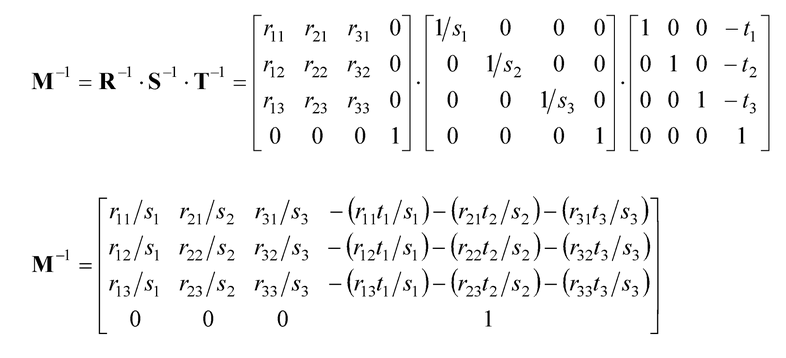
\includegraphics[scale=0.6]{q4.png}
    \end{center}

\end{frame}

\section{Question 5}

\begin{frame}
    \frametitle{Question 5}
    
    Let $M_1 = TR$. \\
    Let $M_2 = RT$. \\
    Is $M_1 = M_2$? Prove it.

\end{frame}

\begin{frame}
    \frametitle{Proof and counterexample}

    \begin{tcolorbox}
        In general $TR \neq RT$.
    \end{tcolorbox}

    i.e. $M_1 \neq M_2$. Counterexample:

    $$T(1, 0, 0) R_z(\pi/2) P(1, 0, 0) \neq R_z(\pi/2) T(1, 0, 0) P(1, 0, 0)$$
    $$P(1, 1, 0) \neq P(0, 2, 0)$$

\end{frame}

\section{Question 6}

\begin{frame}
    \frametitle{Question 6}

    The computation of $\sin \theta$ and $\cos \theta$ is considered relatively slow 
    for some real-time rendering applications. \\

    \vspace{1em}

    However, when the angle $\theta$ is very small, we can make use of the small-angle 
    approximation: $\sin \theta \approx \theta$, and $\cos \theta \approx 1 - \theta_{small}/2$, 
    for better speed.\\

    \vspace{1em}
    
    Write the 4x4 matrix for rotation about the z-axis by a very small rotation angle $\theta_{small}$, 
    which is given in radians. 

\end{frame}

\begin{frame}
    \frametitle{Substitute in}

    \begin{center}
        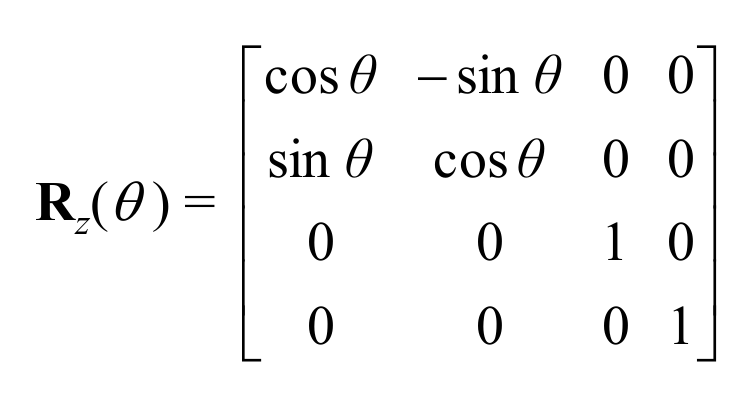
\includegraphics[scale=0.3]{rot-mat.png}
    \end{center}
    
    \begin{tcolorbox}
        $$ \cos \theta \approx 1 - \theta_{small}/2 $$
        $$ \sin \theta \approx \theta_{small} $$
    \end{tcolorbox}

\end{frame}

\section{Question 7}

\begin{frame}
    \frametitle{Question 7}

    In OpenGL, what is the purpose of transforming vertices to window space?

\end{frame}

\begin{frame}
    \frametitle{For the rasterizer!}

    \begin{center}
        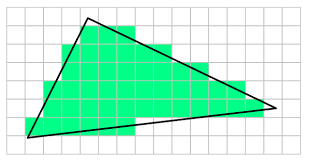
\includegraphics[scale=0.6]{rasterizer.png}
    \end{center}

\end{frame}

\section{Question 8}

\begin{frame}
    \frametitle{Question 8}

    \begin{center}
        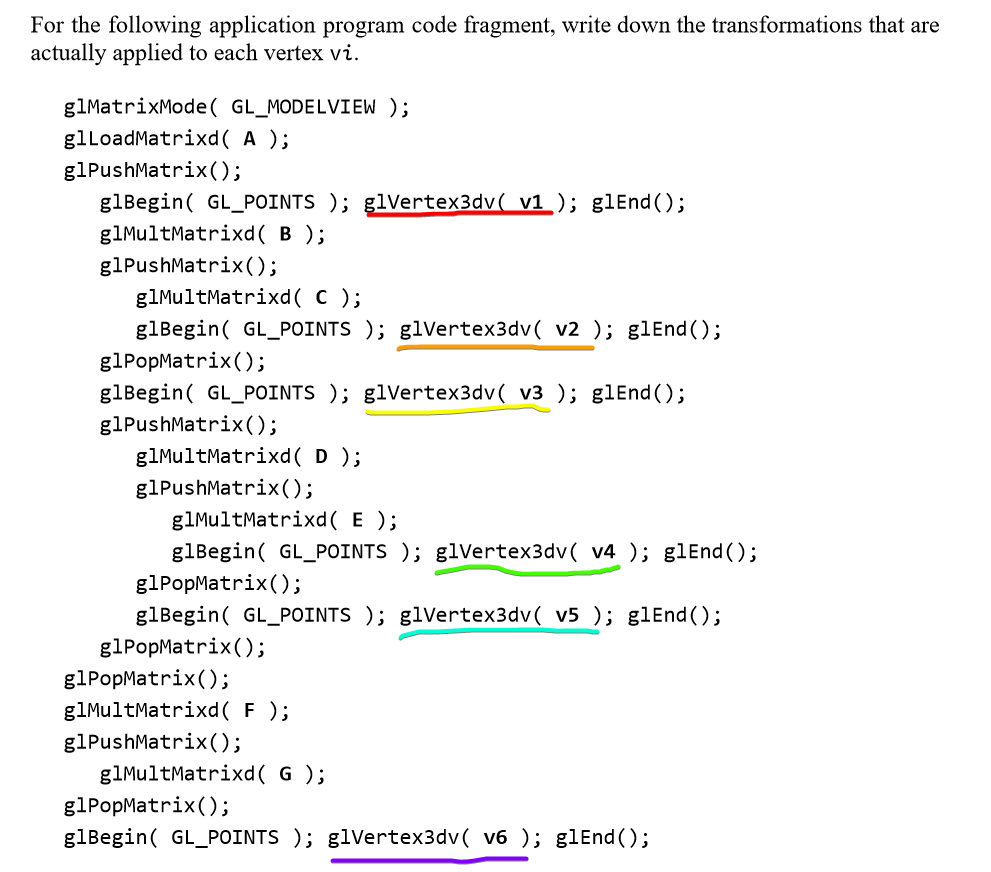
\includegraphics[scale=0.5]{q8.png}
    \end{center}

\end{frame}

\begin{frame}[plain,standout]
    \AlegreyaExtraBold \LARGE
    Attendance taking
\end{frame}

\ThankYou
\begin{frame}[plain,standout]
    Thanks! Get the slides here after the tutorial.\\
    \vspace{2em}
    \scalebox{3}{\faGithub}\par\bigskip
    \url{https://trxe.github.io/cs3241-notes}
\end{frame}

\end{document}